
\documentclass{beamer}
\usecolortheme{dove}
\setbeamertemplate{navigation symbols}{}
\usepackage{amsmath,amssymb,amsfonts,amsthm, multicol, subfigure, color}
\usepackage{bm}
\usepackage{graphicx}
\usepackage{tabularx}
\usepackage{booktabs}
\usepackage{hyperref}
\usepackage{pdfpages}
\usepackage{xcolor}
\definecolor{seagreen}{RGB}{46, 139, 87}
\definecolor{mustard}{RGB}{234, 170, 0}
\def\independenT#1#2{\mathrel{\rlap{$#1#2$}\mkern2mu{#1#2}}}
\newcommand\indep{\protect\mathpalette{\protect\independenT}{\perp}}
\def\log{\text{log}}
\newcommand\logit{\text{logit}}
\newcommand\iid{\stackrel{\text{iid}}{\sim}}
\newcommand\E{\text{E}}
\newcommand\V{\text{V}}
\renewcommand\P{\text{P}}
\newcommand{\Cov}{\text{Cov}}
\newcommand{\Cor}{\text{Cor}}
\newcommand\doop{\texttt{do}}
\usepackage{stackrel}
\usepackage{tikz}
\usetikzlibrary{arrows,shapes.arrows,positioning,shapes,patterns,calc}
\newcommand\slideref[1]{\vskip .1cm \tiny \textcolor{gray}{{#1}}}
\newcommand\red[1]{\color{red}#1}
\newcommand\blue[1]{\color{blue}#1}
\newcommand\gray[1]{\color{gray}#1}
\newcommand\seagreen[1]{\color{seagreen}#1}
\newcommand\purple[1]{\color{purple}#1}
\newcommand\orange[1]{\color{orange}#1}
\newcommand\black[1]{\color{black}#1}
\newcommand\white[1]{\color{white}#1}
\newcommand\teal[1]{\color{teal}#1}
\newcommand\magenta[1]{\color{magenta}#1}
\newcommand\Fuchsia[1]{\color{Fuchsia}#1}
\newcommand\BlueGreen[1]{\color{BlueGreen}#1}
\newcommand\bblue[1]{\textcolor{blue}{\textbf{#1}}}
\newcommand\bred[1]{\textcolor{red}{\textbf{#1}}}
\newcommand\bgray[1]{\textcolor{gray}{\textbf{#1}}}
\newcommand\bgreen[1]{\textcolor{seagreen}{\textbf{#1}}}
\newcommand\bref[2]{\href{#1}{\color{blue}{#2}}}
\colorlet{lightgray}{gray!40}
\pgfdeclarelayer{bg}    % declare background layer for tikz
\pgfsetlayers{bg,main} % order layers for tikz
\newcommand\mycite[1]{\begin{scriptsize}\textcolor{darkgray}{(#1)}\end{scriptsize}}
\newcommand{\tcframe}{\frame{
%\small{
\only<1|handout:0>{\tableofcontents}
\only<2|handout:1>{\tableofcontents[currentsubsection]}}
%}
}

\newcommand{\goalsframe}{\begin{frame}{Goals of the course}

\begin{itemize}
\item connect theories about inequality\\to quantitative empirical evidence
\item evaluate the effects of hypothetical\\interventions to reduce inequality
\item conduct data analysis using the R\\programming language
\end{itemize}
\end{frame}}

\usepackage[round]{natbib}
\bibliographystyle{humannat-mod}
\setbeamertemplate{enumerate items}[default]
\usepackage{mathtools}

\title{Studying Social Inequality with Data Science}
\author{Ian Lundberg}
\date{\today}

\begin{document}

\begin{frame}
\begin{tikzpicture}[x = \textwidth, y = \textheight]
\node at (0,0) {};
\node at (1,1) {};
\node[anchor = north west, align = left, font = \huge] at (0,.9) {Social Data Science};
\node[anchor = north east, align = right] (number) at (1,.9) {};
\node[anchor = north, font = \Large, align = left] at (.5,.5) {\bblue{Course Recap}};
\end{tikzpicture}
\end{frame}

\goalsframe

\begin{frame}{Structure of the Course}
We learned key concepts in social data science.
\begin{enumerate}
\item Population Sampling
\item Models for Subgroup Summaries
\item Causal Inference
\end{enumerate}
\end{frame}

\begin{frame}
\huge Population Sampling
\end{frame}

\begin{frame}
\begin{tikzpicture}[x = \textwidth, y = .8\textheight]
\node (full) at (.25,.5) {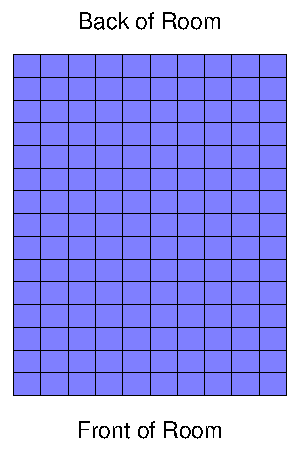
\includegraphics{figures/fullcount}};
\node<1> (srs) at (.75,.5) {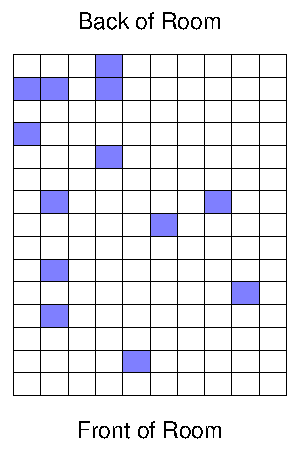
\includegraphics{figures/srs1}};
\node<2> (srs) at (.75,.5) {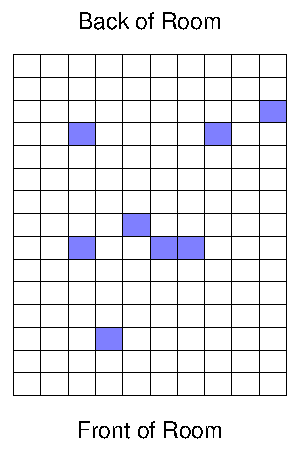
\includegraphics{figures/srs2}};
\node<3> (srs) at (.75,.5) {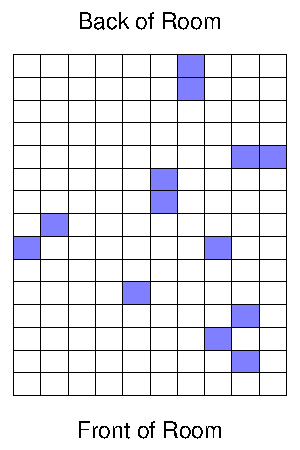
\includegraphics{figures/srs3}};
\node[anchor = south, align = center, font = \bf] at (full.north) {Full Count\\Enumeration};
\node[anchor = south, align = center, font = \bf] at (srs.north) {Probability\\Sample};
\end{tikzpicture}
\end{frame}

\begin{frame}%{Unequal probability sampling}
\begin{tikzpicture}[x = \textwidth, y = .8\textheight]
\node (design) at (.25,.5) {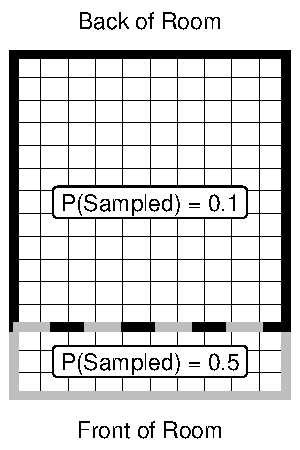
\includegraphics{figures/unequal}};
\node<1> (sample) at (.75,.5) {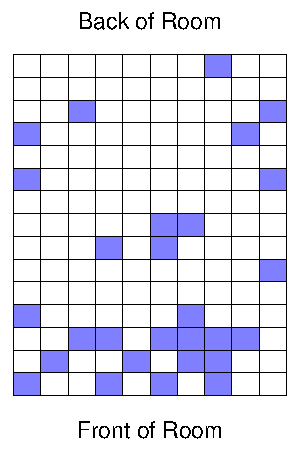
\includegraphics{figures/unequal1}};
\node<2> (sample) at (.75,.5) {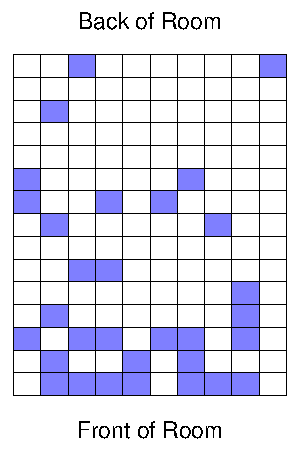
\includegraphics{figures/unequal2}};
\node<3> (sample) at (.75,.5) {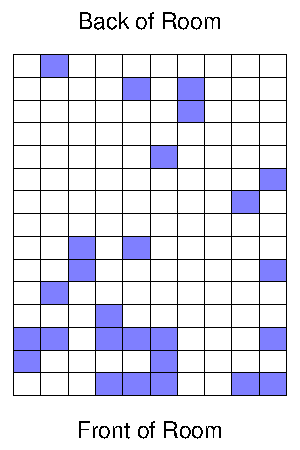
\includegraphics{figures/unequal3}};
\node[anchor = south, align = center, font = \bf] at (design.north) {Sample Design};
\node[anchor = south, align = center, font = \bf] at (sample.north) {Sample};
\end{tikzpicture}
\end{frame}

\begin{frame}{Working with data}
\begin{itemize}
\item Creating objects in R
\item Piping data into functions
\item Summarizing a sample
\item Visualizing with ggplot
\end{itemize}
\end{frame}

\begin{frame}{Working with data}

\Large 
Questions of the form: \vskip .1in
Among \_\_\_\_\_, what is the mean of \_\_\_\_\_? \vskip .3in (population inference from a sample)

\end{frame}

\begin{frame}{Models for Subgroup Summaries}

With only the sample, estimate the mean salary of the Dodgers \vskip .2in

\begin{tabular}{ll}
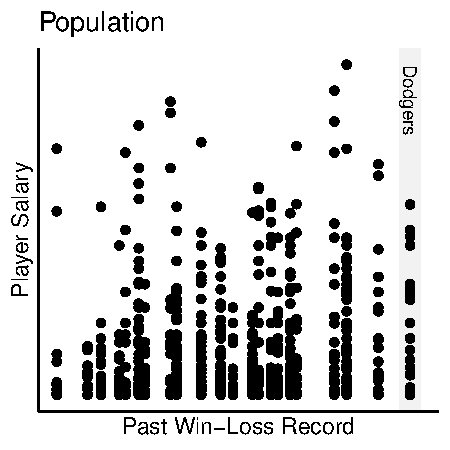
\includegraphics[width = .48\textwidth]{figures/dodgers_population} &
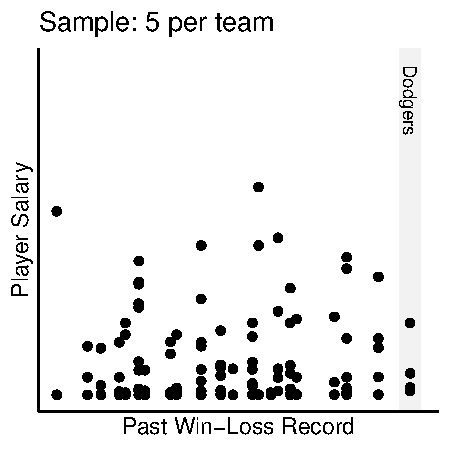
\includegraphics[width = .48\textwidth]{figures/dodgers_sample}
\end{tabular}

\end{frame}

\begin{frame}{Working with Data: Statistical Learning}

\includegraphics<1>[width = \textwidth]{figures/dodgers_estimator1}
\includegraphics<2>[width = \textwidth]{figures/dodgers_estimator2}
\includegraphics<3>[width = \textwidth]{figures/dodgers_estimator3}
\only<4->{
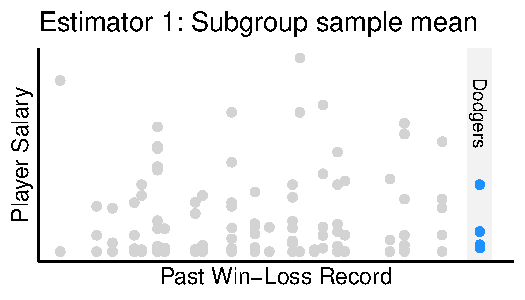
\includegraphics[width = .32\textwidth]{figures/dodgers_estimator1}
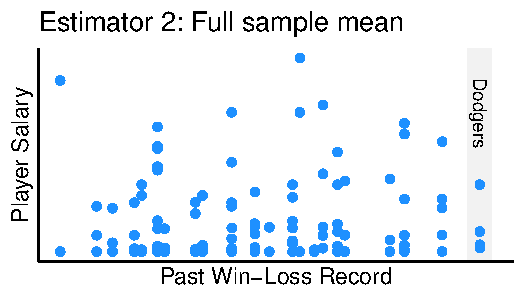
\includegraphics[width = .32\textwidth]{figures/dodgers_estimator2}
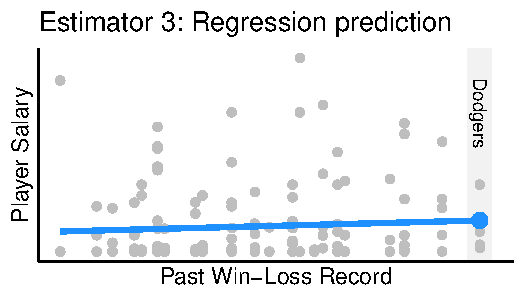
\includegraphics[width = .32\textwidth]{figures/dodgers_estimator3} \vskip .2in
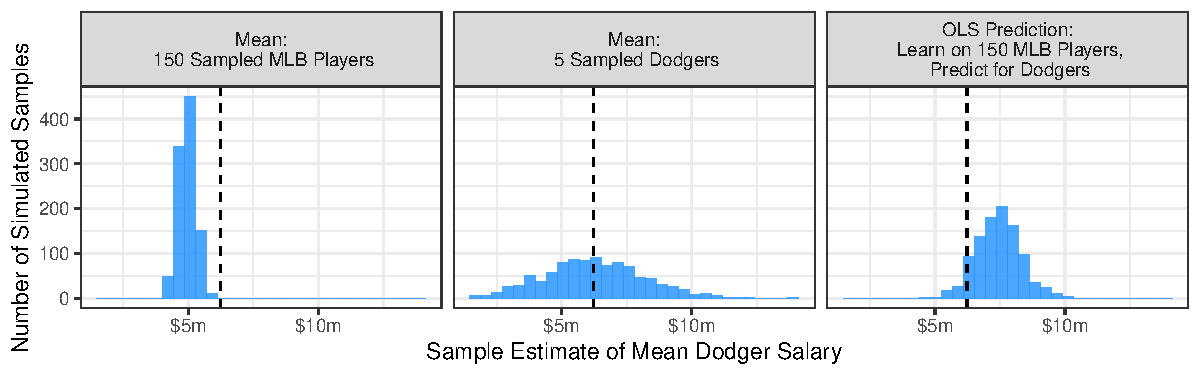
\includegraphics[width = \textwidth]{figures/dodgers_estimator_histogram}
}
\end{frame}

\begin{frame}{Working with Data: Statistical Learning}

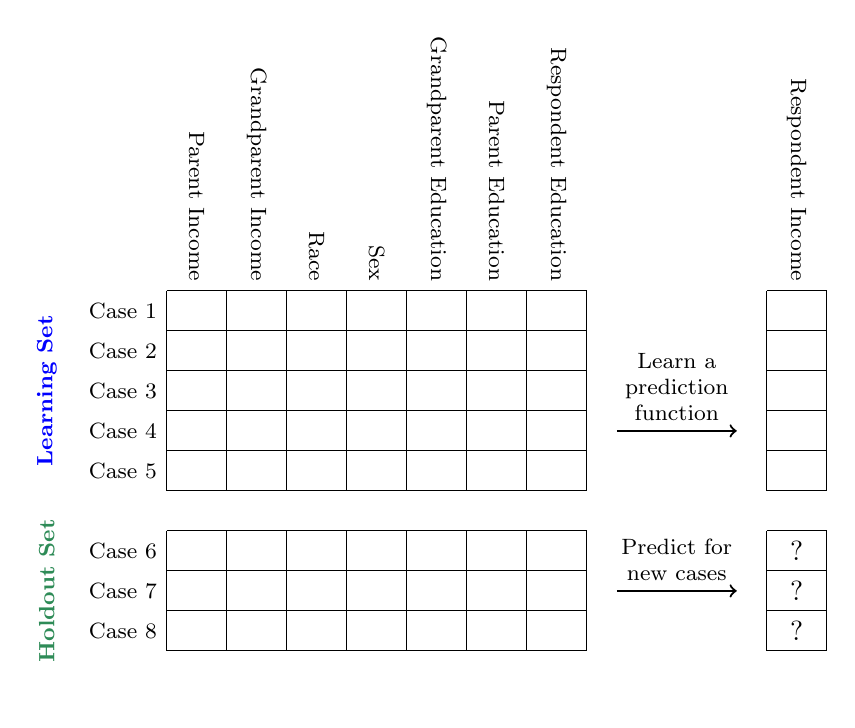
\begin{tikzpicture}[x = 3in, y = 2in]
\node[anchor = east, rotate = 270, font = \footnotesize] at (.15,1) {Parent Income};
\node[anchor = east, rotate = 270, font = \footnotesize] at (.25,1) {Grandparent Income};
\node[anchor = east, rotate = 270, font = \footnotesize] at (.35,1) {Race};
\node[anchor = east, rotate = 270, font = \footnotesize] at (.45,1) {Sex};
\node[anchor = east, rotate = 270, font = \footnotesize] at (.55,1) {Grandparent Education};
\node[anchor = east, rotate = 270, font = \footnotesize] at (.65,1) {Parent Education};
\node[anchor = east, rotate = 270, font = \footnotesize] at (.75,1) {Respondent Education};
\node[anchor = east, font = \footnotesize] at (.1,.95) {Case 1};
\node[anchor = east, font = \footnotesize] at (.1,.85) {Case 2};
\node[anchor = east, font = \footnotesize] at (.1,.75) {Case 3};
\node[anchor = east, font = \footnotesize] at (.1,.65) {Case 4};
\node[anchor = east, font = \footnotesize] at (.1,.55) {Case 5};
\draw[step=.1,black,thin] (0.1,.5) grid (.8,1); 
\node at (.5,1) {};
\node[anchor = east, rotate = 270, font = \footnotesize] at (1.15,1) {Respondent Income};
\draw[step=.1,black,thin] (1.1,.5) grid (1.2,1);
\draw[thin] (1.2,.5) -- (1.2,1);
\draw[->, thick] (.85,.65) -- node[midway, above, font = \footnotesize, align = center] {Learn a\\prediction\\function} (1.05,.65);
% Holdout set
\draw[step=.1,black,thin] (0.1,.1) grid (.8,.4);
\draw[step=.1,black,thin] (1.1,.1) grid (1.2,.4);
\draw[thin] (1.2,.1) -- (1.2,.4);
\node at (1.15,.35) {?};
\node at (1.15,.25) {?};
\node at (1.15,.15) {?};
\node[anchor = east, font = \footnotesize] at (.1,.35) {Case 6};
\node[anchor = east, font = \footnotesize] at (.1,.25) {Case 7};
\node[anchor = east, font = \footnotesize] at (.1,.15) {Case 8};
\draw[->, thick] (.85,.25) -- node[midway, above, font = \footnotesize, align = center] {Predict for\\new cases} (1.05,.25);
% Label the two
\node[rotate = 90, font = {\footnotesize\bf}, blue] at (-.1,.75) {{Learning} Set};
\node[rotate = 90, font = {\footnotesize\bf}, seagreen] at (-.1,.25) {{Holdout} Set};
\node at (-.05,0) {};
\end{tikzpicture}
\end{frame}

\begin{frame}
\huge Causal inference
\end{frame}

\begin{frame}
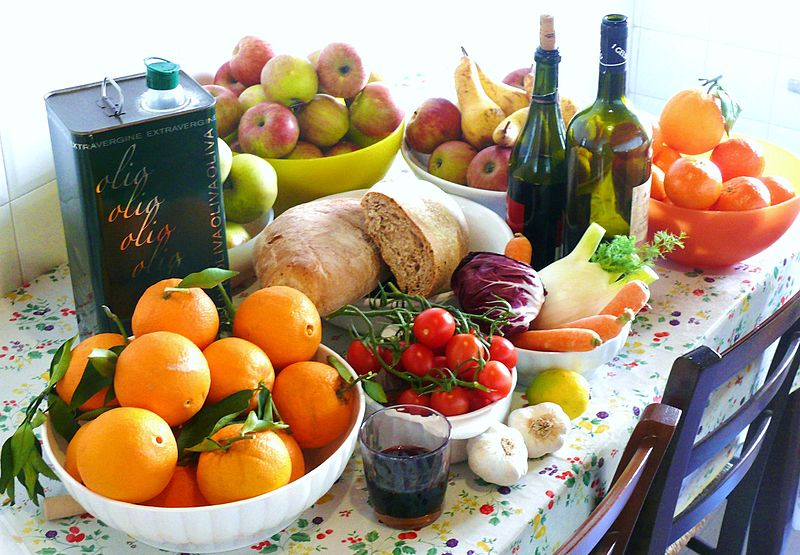
\includegraphics[width = \textwidth]{figures/mediterranean_diet}
\end{frame}

\begin{frame}{Fundamental problem of causal inference}{\href{https://www.tandfonline.com/doi/abs/10.1080/01621459.1986.10478354}{Holland 1986}}

\begin{tikzpicture}[x = \textwidth, y = .8\textheight]
\node at (0,0) {};
\node at (1,1) {};
% Factual outcomes
\node[anchor = north, align = center] at (.25,1) {Descriptive evidence};
\foreach \i in {1,...,8} {
	\node[font = \tiny, anchor = west] at (-.05,9/20-\i/20 + .175) {Person \i};
}
\foreach \i in {.2,.3,.35,.45,.55} {
	\draw[fill = blue, opacity = .3, color = blue] (.05,\i) rectangle (.25,\i + .05) {};
	\node[font = \tiny] at (.15,\i + .025) {lifespan};
}
\foreach \i in {.25,.4,.5} {
	\draw[fill = seagreen, opacity = .3, color = seagreen] (.25,\i) rectangle (.45,\i + .05) {};
	\node[font = \tiny] at (.35,\i + .025) {lifespan};
}
\node[font = \footnotesize, align = center, fill = blue, fill opacity = .3, text opacity = 1] at (.15,.8) {average\\lifespan};
\node[font = \footnotesize, align = center, fill = seagreen, fill opacity = .3, text opacity = 1] at (.35,.8) {average\\lifespan};
\node at (.25,.8) {$-$};
%\node[font = \tiny] at (.15,.575) {$Y_1^\text{Mediterranean Diet}$};
%\node[font = \tiny] at (.35,.525) {$Y_2^\text{Standard Diet}$};
%\node[font = \tiny] at (.15,.475) {$Y_3^\text{Mediterranean Diet}$};
%\node[font = \tiny] at (.35,.425) {$Y_4^\text{Standard Diet}$};
%\node[font = \tiny] at (.15,.375) {$Y_5^\text{Mediterranean Diet}$};
%\node[font = \tiny] at (.15,.325) {$Y_6^\text{Mediterranean Diet}$};
%\node[font = \tiny] at (.35,.275) {$Y_7^\text{Standard Diet}$};
%\node[font = \tiny] at (.15,.225) {$Y_8^\text{Mediterranean Diet}$};
\node[anchor = north, align = center, font = \footnotesize, blue] at (.15, .2) {Outcome\\under\\Mediterranean\\diet};
\node[anchor = north, align = center, font = \footnotesize, seagreen] at (.35, .2) {Outcome\\under\\standard\\diet};
% Potential outcomes
\node[anchor = north, align = center] at (.75,1) {Causal claim};
\node[font = \footnotesize, align = center, fill = blue, fill opacity = .3, text opacity = 1] at (.65,.8) {average\\lifespan};
\node[font = \footnotesize, align = center, fill = seagreen, fill opacity = .3, text opacity = 1] at (.85,.8) {average\\lifespan};
\node at (.75,.8) {$-$};
\foreach \i in {.2,.25,.3,.35,.4,.45,.5,.55} {
	\draw[fill = blue, opacity = .3, color = blue] (.55,\i) rectangle (.75,\i + .05) {};
	\draw[fill = seagreen, opacity = .3, color = seagreen] (.75,\i) rectangle (.95,\i + .05) {};
	\node[font = \tiny] at (.65,\i + .025) {lifespan};
	\node[font = \tiny] at (.85,\i + .025) {lifespan};
}
\node[anchor = north, align = center, font = \footnotesize, blue] at (.65, .2) {Outcome\\under\\Mediterranean\\diet};
\node[anchor = north, align = center, font = \footnotesize, seagreen] at (.85, .2) {Outcome\\under\\standard\\diet};
\foreach \i in {.2,.3,.35,.45,.55} {
	\node[font = \tiny, red] at (.35,\i + .025) {missing};
}
\foreach \i in {.25,.4,.5} {
	\node[font = \tiny, red] at (.15,\i + .025) {missing};
}
\node at (.5,.66) {Causal inference is a \bred{missing data} problem};
\end{tikzpicture}
\end{frame}

\begin{frame}{Potential outcomes}

\begin{huge}
\centering
$$Y_i^a$$
\end{huge}
the outcome $Y$\\
of person $i$\\
if exposed to treatment $A = a$

\end{frame}

\begin{frame}{Causal identification with DAGs}

\begin{figure}
\begin{tikzpicture}[x = \textwidth, y = .8\textheight]
\node (a) at (.5, .45) {$A$};
\node (l) at (.3, .45) {$L$};
\node (y) at (.7, .45) {$Y$};
\draw[->, thick] (a) -- (y);
\draw[->, thick, red] (l) to[out = 45, in = 135] (y);
\draw[->, thick, red] (l) -- (a);
\end{tikzpicture}
\end{figure}
{\color{red} Non-causal path} starts with an edge pointing in to $A$ and ends at $Y$


\vspace{1em}
Identified cusal effects by an adjustment set that blocks all non-causal paths.
\end{frame}

\begin{frame}{Estimation}

\begin{itemize}
\item regression
\item inverse probability weighting
\item matching
\end{itemize}

\end{frame}

\begin{frame}{Causal inference with unmeasured confounding}

\end{frame}

\begin{frame}{Causal inference with unmeasured confounding}
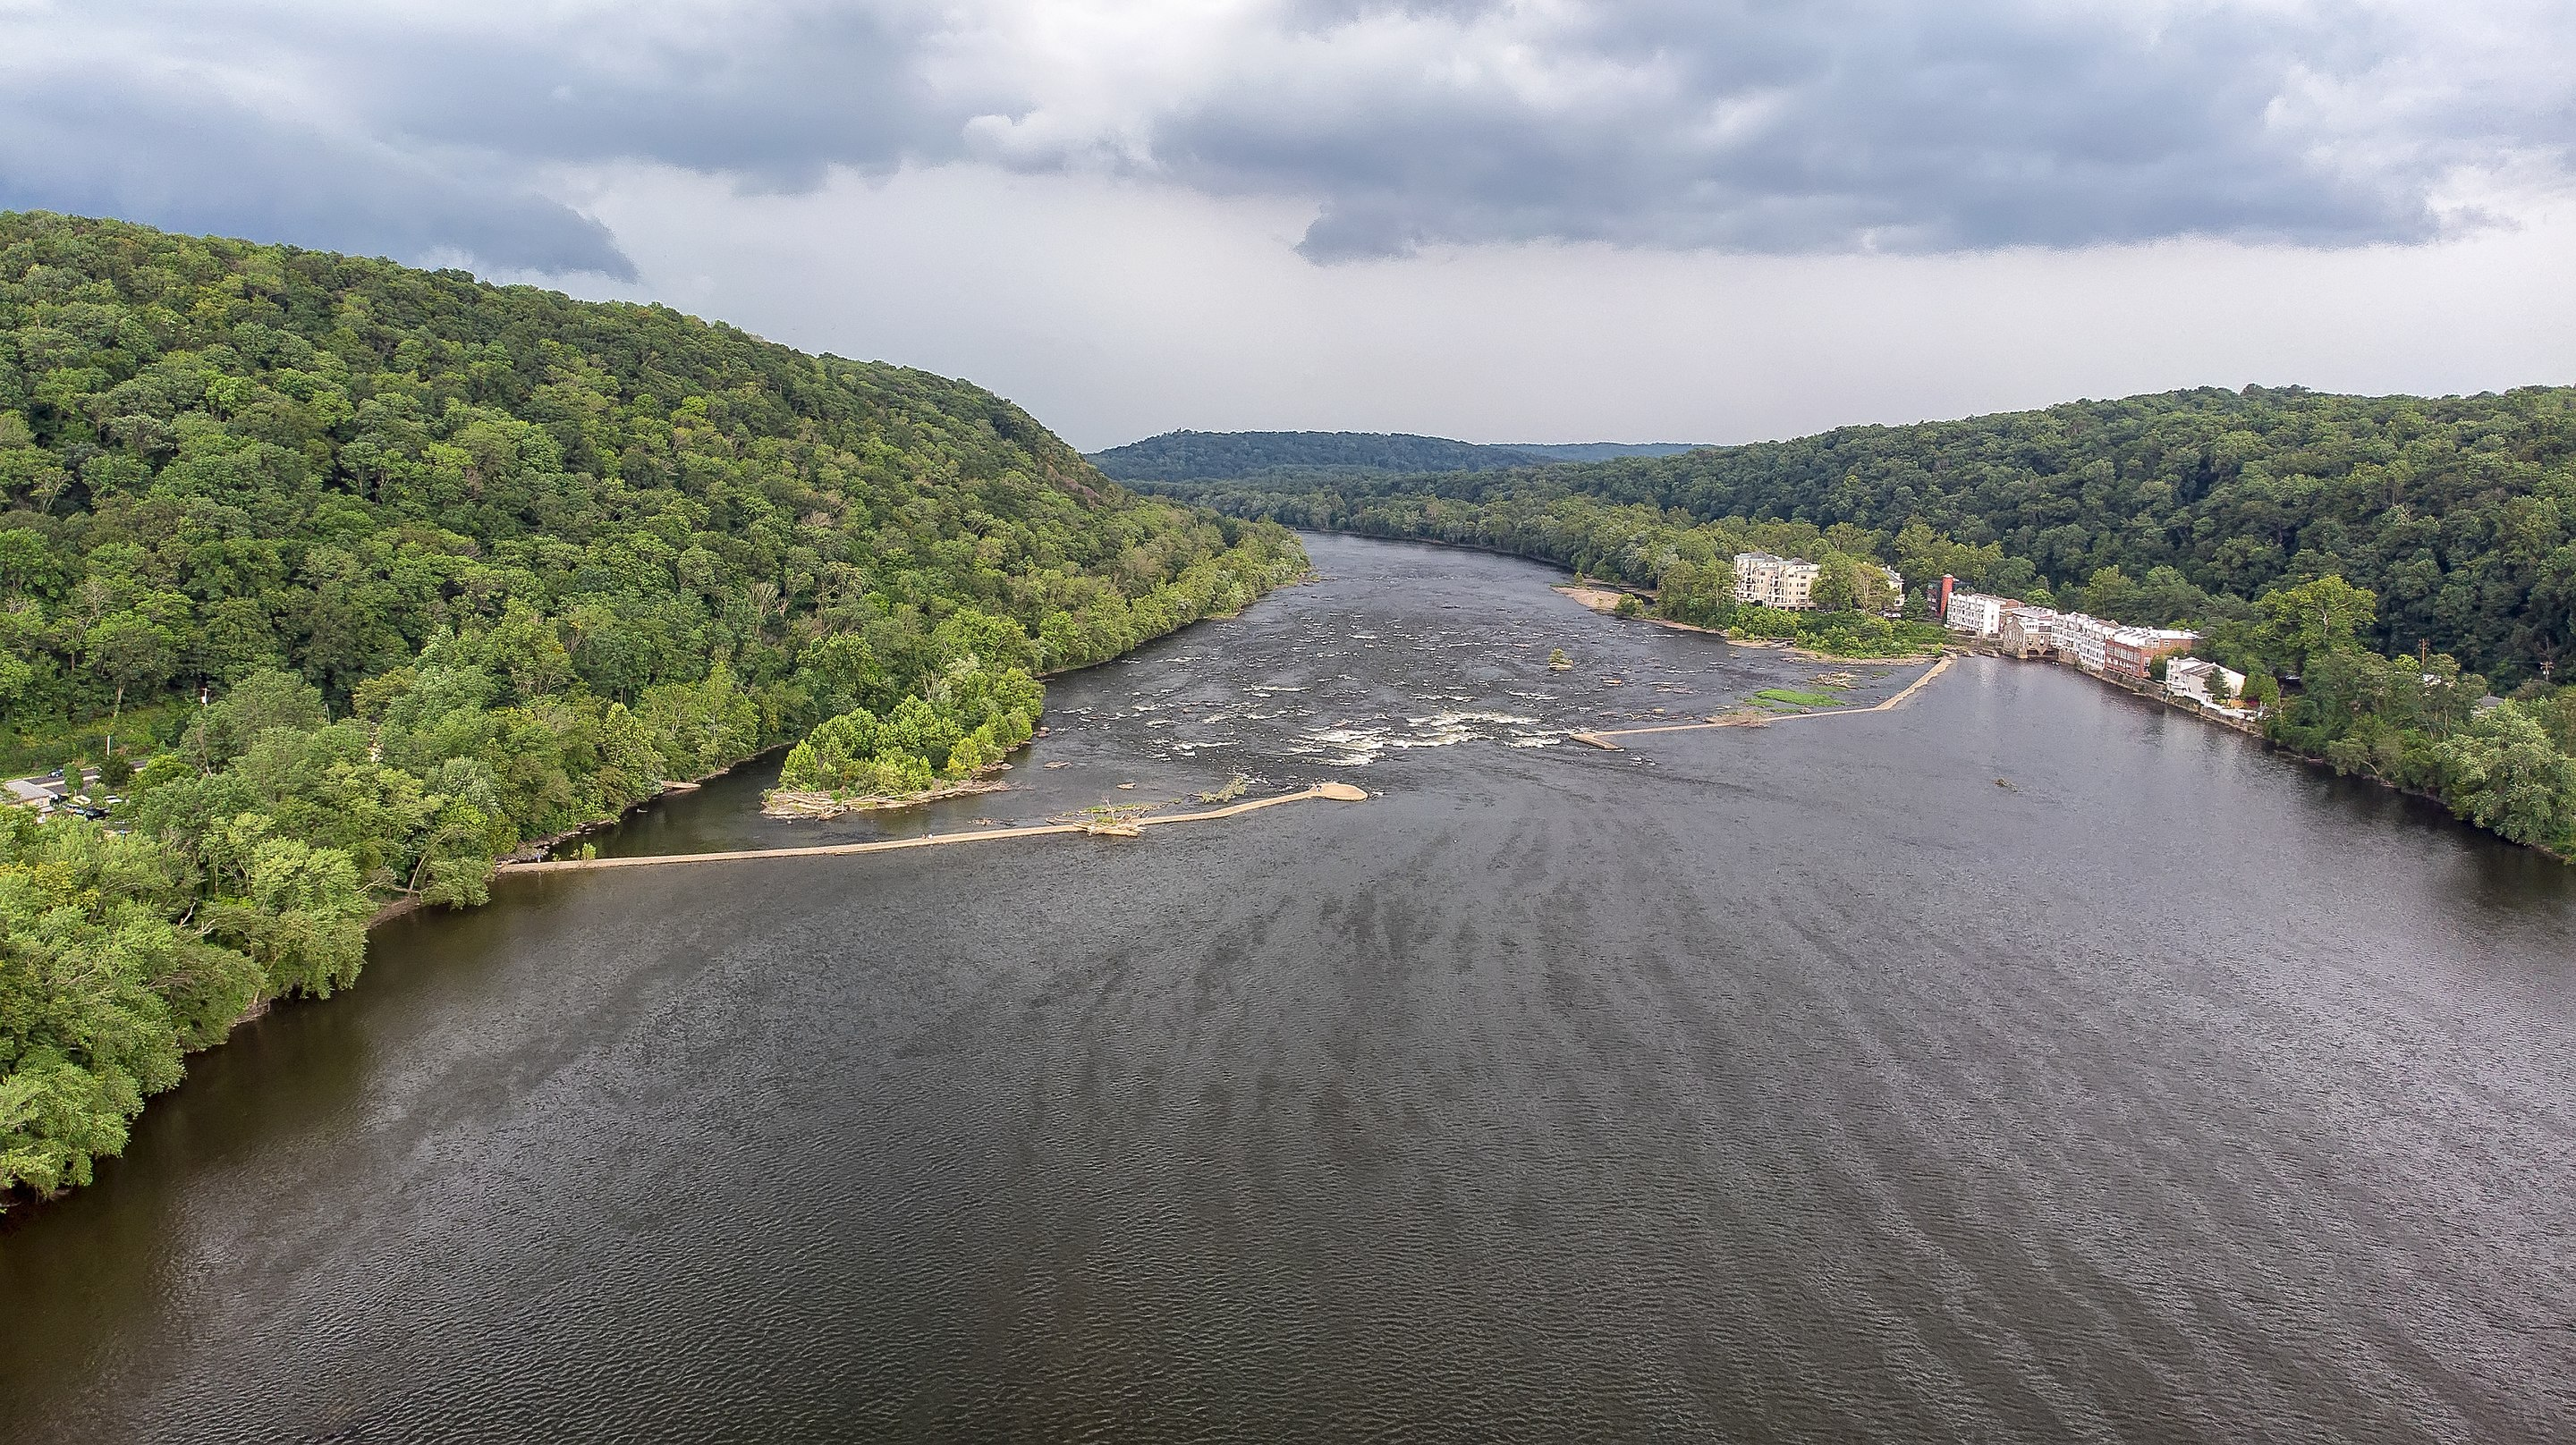
\includegraphics[width = \textwidth]{figures/Delaware_River.jpeg}
\end{frame}

\begin{frame}{Causal inference with unmeasured confounding}
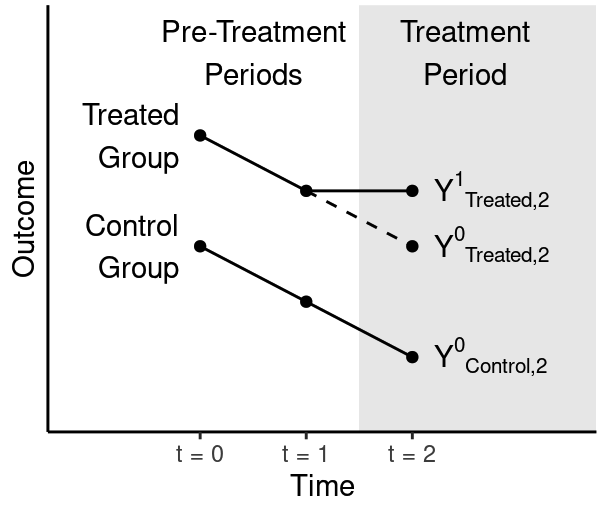
\includegraphics[width = .5\textwidth]{figures/did_from_hw}
\end{frame}

\begin{frame}{Causal inference with unmeasured confounding}
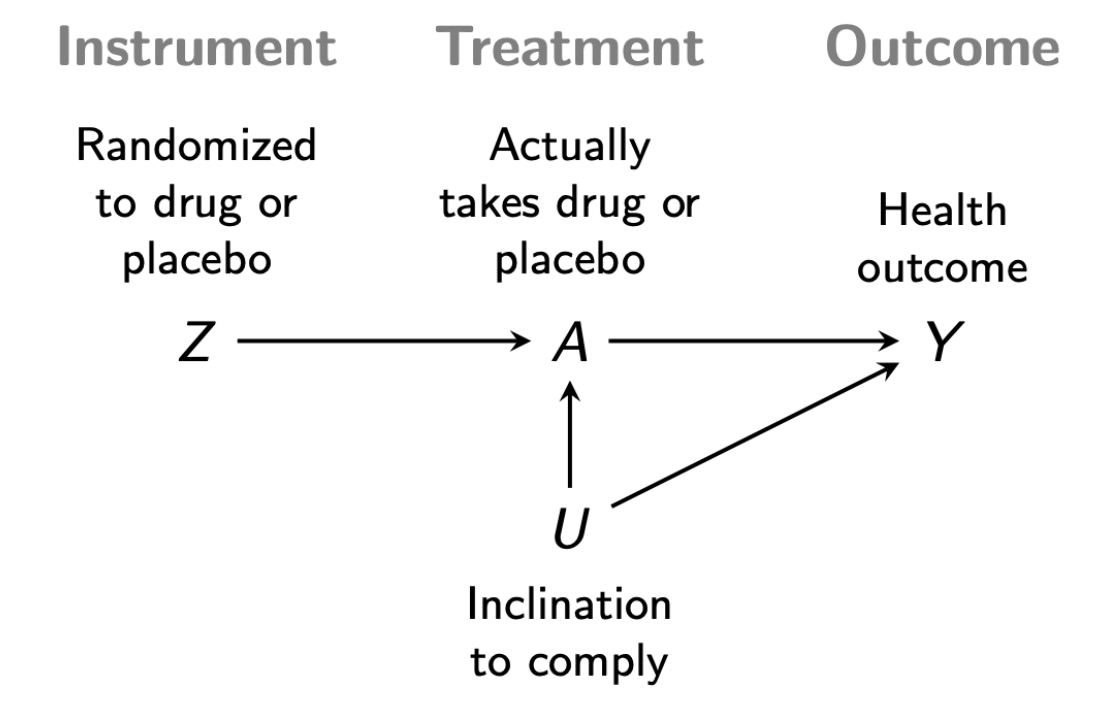
\includegraphics[width = .5\textwidth]{figures/iv_dag}
\end{frame}

\begin{frame}{Course structure}

\begin{itemize}
\item concepts introduced in lecture
\item conceptual practice with quizzes
\item coding practice with problem sets
\item support in office hours and on Piazza
\end{itemize} %\vskip .2in

%
\includegraphics[width = \textwidth]{figures/website_p1}

\end{frame}

\goalsframe

\begin{frame}{Your thoughts}
\begin{itemize}
\item What could we do to make this course better?
\item What is your favorite thing you learned?
\item What parts do you anticipate being most useful for your future work?
\end{itemize}
\end{frame}

%\begin{frame}
%\includegraphics[width = \textwidth]{figures/dag_slide}
%\end{frame}

\begin{frame}{Course evaluations}

\begin{itemize}
\item Specific examples are especially helpful
\begin{itemize}
\item Comments on course content
\item Comments on course delivery
\end{itemize}
\item Specific positive experiences with your TA!
\end{itemize}

\end{frame}

\end{document}